\documentclass[letterpaper,12pt]{article}
\usepackage[utf8]{inputenc}
\usepackage[ngerman]{babel}
\usepackage[rmargin=2.00cm,lmargin=1.5cm,tmargin=2.5cm,bottom=2.00cm]{geometry}
\usepackage[dvipsnames]{xcolor}
\usepackage{fancyhdr}
    \pagestyle{fancy}
    \lhead{{Rodriguez Vega Nayeli}}
\usepackage[dvipsnames]{xcolor}
\usepackage{amsmath}
\usepackage{amssymb}
\usepackage{mathrsfs}
\usepackage{wasysym}
\usepackage{textcomp}
\usepackage{array}
\usepackage{multirow}
\usepackage{mleftright}
\usepackage{graphicx}
%------------
\begin{document}
\pagecolor{pink}

%---------------------------------
\begin{center}
    {\underline{\textbf{\textsc{\Huge{\textcolor{blue}{Tarea 5 -} \textcolor{cyan}{Problemas físicos}}}}}}
\end{center}

\begin{center}
    {\textit{\textcolor{violet}{\textsc{Rodriguez Vega Nayeli}}}}
\end{center}
%-----------------------
\section{Problemas}
\begin{enumerate}
    \item Considerando un sistema en una dimención y sabiendo que $a=\frac{dv}{dt}$ y $v=\frac{dx}{dt}$.Demuestre que la posició se puede ver como:
   \begin{equation}
    x=x_0+v_0t+\frac{1}{2}at^{2} 
    \end{equation}
    
    Para un tiempo inicial $t_0=0$ y con; $x_0$ y $v_0$ la posición y velocidad inicial en el sistema.
%-----------------------

\textcolor{cyan}{Demostración.} Sabemos que...
\begin{equation}
    a=\frac{dv}{dt}
\end{equation}
\begin{equation}
    v=\frac{dx}{dt}
\end{equation}
Entonces para obtener la ecuación de la velocidad, debemos integrar la \textcolor{blue}{\textit{ecuación 2}}
  $$\int_{t_0}^{t} \frac{d\Vec{v}}{dt}dt=\int_{t_0}^{t}\Vec{a_0}dt \Rightarrow por\ el\ teorema\ del\ cambio\ devariable\ \int_{\Vec {v_0}}^{\Vec {v(t)}} d\Vec v=\int_{\Vec {t_0}}^{t} \Vec a_0  \Rightarrow por\ la\ regla $$
  $$de\ Barrow\ \Vec {v_0}\mid _{\Vec {v_0}}^{\Vec {v_{(t)}}}= \Vec{a}t \mid _{t_0}^{\Vec {t}}$$
  
Por lo tanto obtenemos la siguente ecuación:
\begin{equation}
    \Vec{v}_{(t)}-\Vec {v_0}=\Vec {a_0}(t-t_0)
\end{equation}
Pero si despejamos $\Vec{v}_{(t)}$ 
\begin{equation}
     \Vec{v}_{(t)}=\Vec {v_0}+\Vec{a_0}(t-t_0)
\end{equation}
No obstate sabemos que $t_0=0$ por lo tanto la \textcolor{blue}{\textit{ecuación 5}} nos quedaria...

\begin{equation}
     \Vec{v}_{(t)} =\Vec {v_0}+\Vec{a_0}(t)
\end{equation}

Si sustituimos en la  \textcolor{blue}{\textit{ecuación 6}} el   $\Vec{v}_{(t)}$ por la \textcolor{blue}{\textit{ecuación 3}} nos quedaria...
\begin{equation}
      \frac{dx}{dt}=\Vec {v_0}+\Vec{a_0}(t)
\end{equation}
Por lo tanto si integramos {\textcolor{blue}{\textit{ecuación 7}}} nos quedaria...

$$\int_{t_0}^{t}\frac{dx}{dt} dt=\int_{t_0}^{t}[\Vec {v_0}+\Vec{a_0}(t)]dt  \Rightarrow  por\ el\ teorema\ del\ cambio\ devariable\ $$ $$\int_{{x_0}}^{{x}} d\Vec{x}=\int_{t_0}^{t}\Vec{v_0} dt+\int_{t_0}^{t}\Vec{a_0}(t)dt  \Rightarrow por\ la\ regla\ de\ Barrow\  {x}\mid _{ {x_0}}^{x}= {\Vec{a}}t \mid _{t_0}^{t}\frac{\Vec{a_0t^{2}}}{2}\mid _{t_0}^{t}$$
Por lo tanto obtenemos la siguiente ecuación.
\begin{equation}
      {x}-{x_0}=\Vec{v_0}(t-t_0)+\frac{\Vec{a}(t-t_0)^{2}}{2}
\end{equation}
Pero si despejamos ${x}$ de la {\textcolor{blue}{\textit{ecuación 8}}} nos quedaria 
\begin{equation}
      {x}={x_0}+\Vec{v_0}(t-t_0)+\frac{1}{2}\Vec{a}(t-t_0)^{2}
\end{equation}
No obstante sabemos que el tiempo es $t_0=0$, la ecuacion {\textcolor{blue}{\textit{ecuación 9}}} nos quedaria 
\begin{equation}
      {x}={x_0}+\Vec{v_0}t+\frac{1}{2}\Vec{a}t^{2}
\end{equation}

$$\therefore {x}={x_0}+\Vec{v_0}t+\frac{1}{2}\Vec{a}t^{2} = {x}={x_0}+\Vec{v_0}t+\frac{1}{2}\Vec{a}t^{2}\blacksquare$$ 
%---------------------------
    \item Considere una carrera entre dos coches, éstos arrancan del reposo pero el coche uno hace trampa (cosa que nunca pasa), saliendo un segundo antes que el segundo, si los autos tienen una aceleración de 3.5m/$s^{2}$ y 4.9m/$s^{2}$ respectivamente. 
     \begin {itemize}
    \item[a)] En que momento el auto dos alcanza al auto uno, i.e. $t =?$
    
    {\textcolor{red}{Datos}}
    
    $\Vec{a}_{auto \ 1}$=3.5m/$s^{2}$
    
    $\Vec{a}_{auto \ 2}$=4.9m/$s^{2}$
    
    $x_{0}$=0m
    
    {\textcolor{red}{Obsevación}}
     
     Sabemos que el tiempo del carro uno es $t_1= t$ pero este salio un segundo antes, por lo tanto podemos determinar que  el tiempo del el carro dos es $t_2=t-1$ 
     
    {\textcolor{red}{Formula / Despejes}} 
    \begin{equation}
      {x}={x_0}+\Vec{v_0}t+\frac{1}{2}\Vec{a}t^{2}
      \end{equation}
     Pero como la $x_0=0$ entonces...
     \begin{equation}
      x=\frac{1}{2}\Vec{a}t^{2}
      \end{equation}
    {\textcolor{red}{Operaciones}} 
    
    {\textcolor{orange}{Carro uno:}} Sabemos que la aceleración $=3.5m/s^{2}$ por lo tanto si lo sustituimos en la $\Vec{a}$ en la {\textcolor{blue}{\textit{ecuación 12}}} nos quedaria...
    \begin{equation}
      x=\frac{3.5m/s}{2}^{2}t^{2}
      \end{equation}
    
     {\textcolor{cyan}{Carro dos:}} Sabemos que la aceleración $=4.9m/s^{2}$ por lo tanto si lo sustituimos en la $\Vec{a}$ en la {\textcolor{blue}{\textit{ecuación 12}}} al igual que  $t$ por $t-1$ nos quedaria...
     
      $$x=\frac{1}{2}\Vec{a}(t)^{2}=\frac{1}{2}4.9m/s^{2}(t-1)^{2} \Rightarrow \frac{4.9m/s^{2}}{2}(t^{2}-2t+1) \Rightarrow \frac{4.9m/s^{2}}{2}t^{2}-\frac{4.9m/s^{2}}{2}(2t)+$$
      
       $$+\frac{4.9m/s^{2}}{2}(+1)\Rightarrow \frac{4.9m/s^{2}}{2}t^{2}-4.9m/s^{2}(t)+\frac{49}{20}m/s^{2}$$
      
     Entonces:
      
     \begin{equation}
      x=\frac{4.9m/s^{2}}{2}t^{2}-4.9m/s^{2}(t)+\frac{49}{20}m/s^{2}
      \end{equation}
     Igualando la {\textcolor{blue}{\textit{ecuación 13}}} con la {\textcolor{blue}{\textit{ecuación 14}}}: 
     
     $$\frac{3.5m/s}{2}^{2}t^{2}=\frac{4.9m/s^{2}}{2}t^{2}-4.9m/s^{2}(t)+\frac{49}{20}m/s^{2}$$
     
      $$0=\frac{4.9m/s^{2}}{2}t^{2}-\frac{3.5m/s}{2}^{2}t^{2}-4.9m/s^{2}(t)+\frac{49}{20}m/s^{2}$$
      
     \begin{equation}
       0=\frac{7}{10}m/s^{2}t^{2}-4.9m/s^{2}(t)+\frac{49}{20}m/s^{2}
      \end{equation}
     Utilizaremos la ecuacion general en la {\textcolor{blue}{\textit{ecuación 15}}} para encontrar $t$
     
     $$t=\frac{-b \pm \sqrt{b^{2}-4ac}}{2a}$$
     
     $$t=\frac{-(-4.9 m/s^{2})\pm \sqrt{(-4.9 m/s^{2})^{2}-4(\frac{7}{10}m/s^{2})(\frac{49}{20})m/s^{2}}}{2(\frac{7}{10}m/s^{2})}$$
     
     $$t=\frac{4.9 m/s^{2}\pm \sqrt{\frac{2401}{100}m^{2}/s^{4}-\frac{343}{50}m^{2}/s^{4}}}{\frac{7}{5}m/s^{2}}$$
     
    $$t=\frac{4.9 m/s^{2}\pm \sqrt{\frac{343}{20}m^{2}/s^{4}}}{\frac{7}{5}m/s^{2}}$$
     
    $$t_1=\frac{4.9 m/s^{2}+ \sqrt{\frac{343}{20}m^{2}/s^{4}}}{\frac{7}{5}m/s^{2}}=6.45s$$
    $$t_2=\frac{4.9 m/s^{2}- \sqrt{\frac{343}{20}m^{2}/s^{4}}}{\frac{7}{5}m/s^{2}}=0.54s$$
    
    Al analizar los resultados podemos observar que tenemos dos resultados, por lo tanto tomaremos el primero ($t_1$) debido a que es imposible que el carro dos lo alcanzara el carro uno en un tiempo de 0.54s.
    
    
    $\therefore$ En el tiempo 6.45s aproximadamente el carro dos alcanzo al auto uno. 
    
     %--------------------------
    \item[b)] Cuál será la posición cuando el inciso (a) ocurra, $x=?$
    
    {\textcolor{red}{Datos}}
    
    $\Vec{a}_{auto \ 1}$=3.5m/$s^{2}$
    
    $\Vec{a}_{auto \ 2}$=4.9m/$s^{2}$
    
    $x_{0}$=0m
    
    $t$=6.45s
    
    {\textcolor{red}{Formula}}
     \begin{equation}
      {x}={x_0}+\Vec{v_0}t+\frac{1}{2}\Vec{a}t^{2}
      \end{equation}
    Pero como la $x_0=0$ y la $v_0=0$ entonces...
    \begin{equation}
      {x}=\frac{1}{2}\Vec{a}t^{2}
      \end{equation}
     {\textcolor{red}{Operaciones}} 
     
     {\textcolor{orange}{Carro uno:}} Sabemos que la aceleración $3.5m/s^{2}$ por lo tanto si lo sustituimos en la $\Vec{a}$ en la {\textcolor{blue}{\textit{ecuación 17}}} tambien sustitimos $t$ por 6.45s y nos quedaria... 
    \begin{equation}
      x=\frac{3.5m/s}{2}^{2}(6.45s)^{2}=\frac{3.5m/s}{2}^{2}\left(\frac{16641}{400}s^{2}\right)=72.80m 
      \end{equation}
     {\textcolor{cyan}{Carro dos:}} Sabemos que la aceleración $4.5m/s^{2}$ por lo tanto si lo sustituimos en la $\Vec{a}$ en la {\textcolor{blue}{\textit{ecuación 17}}} tambien sustitimos $t$ por (6.45s-1s) y nos quedaria... 
     \begin{equation}
      x=\frac{4.9m/s}{2}^{2}(6.45s-1s)^{2}=\frac{4.9m/s}{2}^{2}(5.45s)^{2}=\frac{4.9m/s}{2}^{2}\left(\frac{11881}{400}s^{2}\right)=72.77m
      \end{equation}
    Por lo tanto si igualamos la {\textcolor{blue}{\textit{ecuación 18}}} y {\textcolor{blue}{\textit{ecuación 19}}} nos daria...
    
    $$72.80m=72.77m \Rightarrow x \approx 72.80m$$
    
    $\therefore$ Cuando el auto dos alcanza al primer carro estara a una distancia de  72.80 m aproximadamente.
     
    \item[c)] Cuál será la velocidad que tendrá en ese punto para ambos autos.
    
    {\textcolor{red}{Datos}}
    
    $\Vec{a}_{auto \ 1}$=3.5m/$s^{2}$
    
    $\Vec{a}_{auto \ 2}$=4.9m/$s^{2}$
    
    $x_{0}$=0m
    
    $t$=6.45s
    
    $x$=72.80m
    
     {\textcolor{red}{Formula}}
      \begin{equation}
      v_f=V_0+at
      \end{equation}
      Pero como $V_0$= 0 entonces...
      \begin{equation}
      v_f=at
      \end{equation}
      {\textcolor{red}{Operacion/Resultado}}
       
       {\textcolor{orange}{Carro uno:}} Sabemos que la aceleración $3.5m/s^{2}$ por lo tanto si lo sustituimos en la $\Vec{a}$ en la {\textcolor{blue}{\textit{ecuación 21}}} tambien sustitimos $t$ por 6.45s y nos quedaria... 
    \begin{equation}
       v_f=(3.5m/s^{2})(6.45s)=22.575m/s
      \end{equation}
     {\textcolor{cyan}{Carro dos:}} Sabemos que la aceleración $4.5m/s^{2}$ por lo tanto si lo sustituimos en la $\Vec{a}$ en la {\textcolor{blue}{\textit{ecuación 21}}} tambien sustitimos $t$ por (6.45s-1s) y nos quedaria... 
     \begin{equation}
      V_f=(4.9m/s^{2})(6.45s-1s)=(4.9m/s^{2})(5.45s)=26.705m/s
      \end{equation}
    
    $\therefore$ El primer auto tienen una velocidad de 22.575m/s aproximadamete y el auto dos tienen una velocidad  de 26.705m/s aproximadamente.
%--------------------- 
     \item[d)]Toma 5 tiempos diferentes a partir de que los autos arrancan, sin tomar el tiempo inicial, 3 antes del tiempo donde los autos se encuentran y dos posteriores a ese tiempo, realicen dos tablas, una para cada auto, con la siguiente información; aceleración, tiempo posición y velocidad como se muestra en el Cuadro 1. 
  \end{itemize} 
  \begin{table}[h]
        \centering
            \begin{tabular}{|c|c|c|c|c|c|}\hline \hline
                \multicolumn{6}{|c|}{Auto 1}\\\hline
                \multicolumn{3}{|l|}{No dependiente del tiempo} & \multicolumn{3}{|l|}{Dependientes del tiempo}\\\hline
                \multicolumn{3}{|c|}{$\vec{a}[m/s^{2}]$}
                & {$t[s]$} & {$\vec{x}[m]$} & {$\vec{v}[m/s]$}\\\hline
                \multicolumn{3}{|c|}{} &3  &15.75  &10.5 \\\cline{4-6}
                \multicolumn{3}{|c|}{} &4  &28  &14 \\\cline{4-6}
                \multicolumn{3}{|c|}{$3.5m/s^{2}$} &5  &43.75  &17.5 \\\cline{4-6}
                \multicolumn{3}{|c|}{} &7  &85.75  &24.5 \\\cline{4-6}
                \multicolumn{3}{|c|}{} &9 &141.75  &31.5 \\\hline \hline
            \end{tabular}\\
        \caption{\textcolor{cyan}{Cinemática del Auto 1}}
        \label{Cuadro 1: Cinemática del Auto 1}
        \end{table}  

%-----------------------------------
{\textcolor{red}{Formula}}

${x}=\frac{1}{2}\Vec{a}t^{2}$

$v_f=V_0+at$
%---------------------------
{\textcolor{red}{Operaciones}}
%------

Cuando el $t=3$ entonces...

$${x}=\frac{1}{2}\Vec{a}t^{2}=\frac{3.5m/s^{2}}{2}(3s)^{2}=15.75m$$

$$v_f=at=3.5m/s^{2}(3s)=10.5m/s$$
%-----
Cuando el $t=4$ entonces...

$${x}=\frac{1}{2}\Vec{a}t^{2}=\frac{3.5m/s^{2}}{2}(4s)^{2}=28m$$

$$v_f=at=3.5m/s^{2}(4s)=14m/s$$
%-----
Cuando el $t=5$ entonces...

$${x}=\frac{1}{2}\Vec{a}t^{2}=\frac{3.5m/s^{2}}{2}(5s)^{2}=43.75m$$

$$v_f=at=3.5m/s^{2}(5s)=17.5m/s$$
%------
Cuando el $t=7$ entonces...

$${x}=\frac{1}{2}\Vec{a}t^{2}=\frac{3.5m/s^{2}}{2}(7s)^{2}=85.75m$$

$$v_f=at=3.5m/s^{2}(7s)=24.5m/s$$
%------
Cuando el $t=9$ entonces...

$${x}=\frac{1}{2}\Vec{a}t^{2}=\frac{3.5m/s^{2}}{2}(9s)^{2}=141.75m$$

$$v_f=at=3.5m/s^{2}(9s)=31.5m/s$$
  \begin{table}[h]
        \centering
            \begin{tabular}{|c|c|c|c|c|c|}\hline \hline
                \multicolumn{6}{|c|}{Auto 2}\\\hline
                \multicolumn{3}{|l|}{No dependiente del tiempo} & \multicolumn{3}{|l|}{Dependientes del tiempo}\\\hline
                \multicolumn{3}{|c|}{$\vec{a}[m/s^{2}]$} & {$t[s]$} & {$\vec{x}[m]$} & {$\vec{v}[m/s]$}\\\hline
                \multicolumn{3}{|c|}{} &3 &22.05  &14.7 \\\cline{4-6}
                \multicolumn{3}{|c|}{} &4  &39.2  &19.6 \\\cline{4-6}
                \multicolumn{3}{|c|}{$4.9m/s^{2}$} &5  &61.25  &24.5 \\\cline{4-6}
                \multicolumn{3}{|c|}{} &7  &120.05  &34.3 \\\cline{4-6}
                \multicolumn{3}{|c|}{} &9  &198.45  &44.1 \\\hline \hline
            \end{tabular}\\
        \caption{\textcolor{cyan}{Cinemática del Auto 2}}
        \label{Cuadro 1: Cinemática del Auto 1}
        \end{table} 
%-----------------------------------
{\textcolor{red}{Formula}}

${x}=\frac{1}{2}\Vec{a}t^{2}$

$v_f=V_0+at$
%---------------------------
{\textcolor{red}{Operaciones}}
%------

Cuando el $t=3$ entonces...

$${x}=\frac{1}{2}\Vec{a}t^{2}=\frac{4.9m/s^{2}}{2}(3s)^{2}=22.05m$$

$$v_f=at=4.9m/s^{2}(3s)=14.7m/s$$
%-----
Cuando el $t=4$ entonces...

$${x}=\frac{1}{2}\Vec{a}t^{2}=\frac{4.9m/s^{2}}{2}(4s)^{2}=39.2m$$

$$v_f=at=4.9m/s^{2}(4s)=19.6m/s$$
%-----
Cuando el $t=5$ entonces...

$${x}=\frac{1}{2}\Vec{a}t^{2}=\frac{4.9m/s^{2}}{2}(5s)^{2}=61.25m$$

$$v_f=at=4.9m/s^{2}(5s)=24.5m/s$$
%------
Cuando el $t=7$ entonces...

$${x}=\frac{1}{2}\Vec{a}t^{2}=\frac{4.9m/s^{2}}{2}(7s)^{2}=120.05m$$

$$v_f=at=4.9m/s^{2}(7s)=34.3m/s$$
%------
Cuando el $t=9$ entonces...

$${x}=\frac{1}{2}\Vec{a}t^{2}=\frac{4.9m/s^{2}}{2}(9s)^{2}=198.45m$$
$$v_f=at=4.9m/s^{2}(9s)=44.1m/s$$
\item[e)]Considere el siguiente sistema, dos bloques de masas $m_1$ y $m_2$ estan unidos por
una cuerda ideal y descansan sobre una superficie horizontal sin roce. Si una fuerza
de magintud A se le aplica al bloque de masa m2 horizontalmente, en la dirección
que muestra la Figura 1. Realicen los respectivos diagramas de cuerpos libres (usen powerpoint, paint,dibujelo, lo que guste) y anexalo como una imagen, apartir de ellos determinen la aceleración del sistema y la tensión de la cuerda entre los bloques.
\begin{figure}[ht]
    \centering
    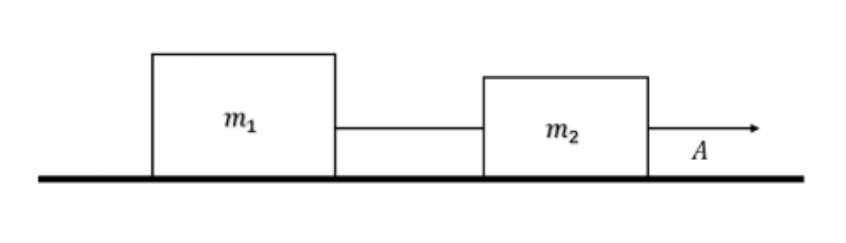
\includegraphics{Imagenes/imafisica.jpg}
    \caption{Sistema de dos bloques amarrados}
    \label{fig:my_label}
\end{figure}

{\textcolor{cyan}{Analisis}}

Al analizar el sistema de dos bloques amarrados, podemos deterninar que los cuerpos esta sometidos por varias fuerzas.De forma paralela esta sometido por la fuerza de la gravedad y la fuerza natural y de forma horizontal podemos decir que la fuerza $A$ actua sobre el bloque de $m_2$ entonces...
$$A-T=ma$$
$$A-T=ma$$
En donde $a$ es la aceleración que experimentan ambos bloques, ya que se mueven a la misma dirección y sentido debido a que estan unidos por la cuerda, por lo tanto al sumar las dos ecuacion nos quedaria que: 
$$A=a(m_1+m_2)$$
$$a=\frac{a}{m_1+m_2}$$
No obstante si queremos calcualar la tensión podemos remplazar la aceleración encontrada en cualquiera de las eciaciones de la fuerza neta, por lo tanto nos quedaria de la siguiente manera...
$$T=\frac{m_1a}{m_1+m_2}$$
No obstante de la forma mas conocida la tension se puede calcular de la siguentes manera.
$$T=ma$$
\begin{figure}[th]
    \centering
    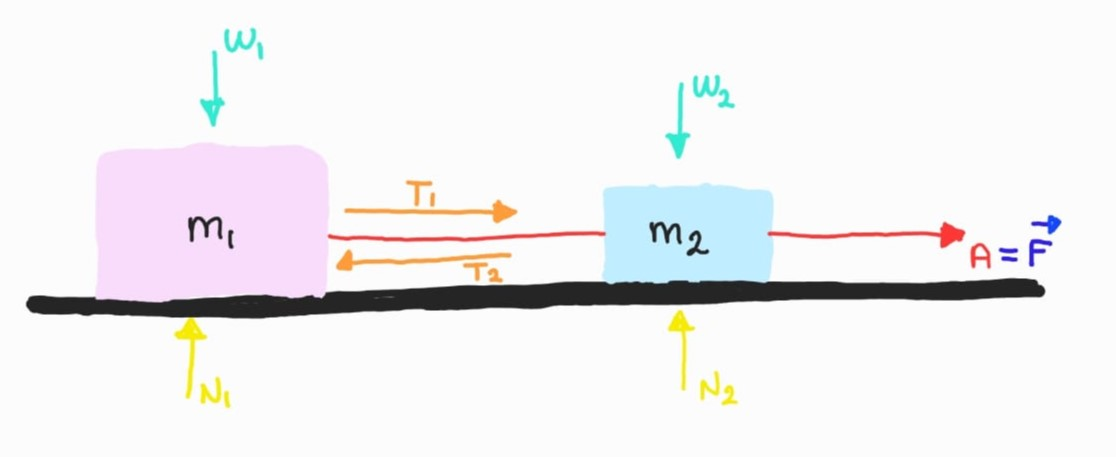
\includegraphics[scale=0.500]{Imagenes/Dibujo del Diagrama.jpeg}
    \caption{Sistema de dos bloques amarrados}
    \label{fig:my_label}
\end{figure}
\end{enumerate}
\end{document}
